\chapter*{3 Versuchsdurchführung und Auswertung}
\addcontentsline{toc}{chapter}{3 Versuchsdurchführung und Auswertung}
\setcounter{chapter}{3}
\setcounter{section}{0}
\setcounter{subsection}{0}

\section{Versuch 1 - Strukturaufklärung}

    \subsection{Versuchsaufbau und -durchführung}

        In diesem Versuch soll die Gitterkonstante $g$ eines optischen Gitters bestimmt werden. Dazu wird ein HeNe-Laser mit einer Wellenlänge von $\lambda = 632,8\ \mathrm{nm}$ verwendet (In allen folgenden Versuchen, in denen ein Laser verwendet wird, handelt es sich um diesen Laser und damit auch um die gleiche Wellenlänge und wird dementsprechen nicht erneut angegeben). Dieser stellt dabei eine kohärente Lichtquelle dar, strahlt also paralleles Licht aus. Dieses
        Licht wird nun senkrecht auf das Gitter gerichtet, welches sich senkrecht zu Wand befindet. Der Wand dient hier als Schirm. Aus der Lage der Beugungsmaxima lässt sich nun bei bekannter Wellenlänge die Gitterkonstante $g$ bestimmten. Dazu wird der Abstand $L$ zwischen Wand und Gitter gemessen und die Abstände zwischen den Beugungsmaxima gleicher Ordnung. Die Gitterkonstante $g$ ergibt sich dann aus der folgenden Formel:

        \begin{equation}
            g = \frac{2 n \lambda L}{a_{n}}
        \end{equation}

        Es kann diese Formel verwendet werden, da die Beugungswinkel sehr klein sind und somit die Kleinwinkelnäherung verwendet werden kann.

        \begin{figure}
            \centering
            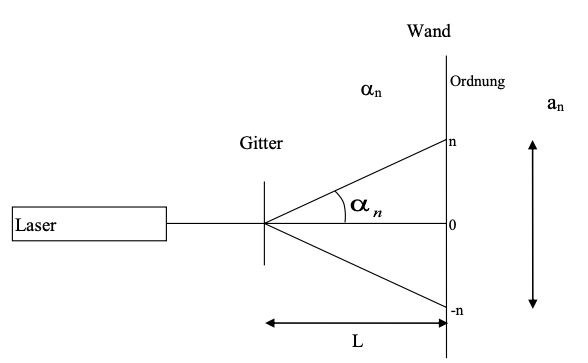
\includegraphics[width=0.5\textwidth]{bilder/Physik_Aufbau_01.png}
            \caption{Versuchsaufbau Versuch 1}
            \label{fig:Versuchsaufbau1}
        \end{figure}
    
    \subsection{Ergebnisse}

        In der folgenden Tabelle sind die Messwerte mit den dazugehörigen Gitterkonstanten aufgelistet. Die Gitterkonstante wurde dabei für die erste und zweite Ordnung bestimmt.

        \begin{table}[H]
            \centering
            \caption{Messwerte Versuch 1}
            \vspace*{1em}
            \begin{tabular}{|l|l|l|l|}
                \hline
                & Abstand $a_{n}$ & Abstand $L$ & Gitterkonstante $g_{n}$\\
                \hline
                $n = 1$ & $19,0\ \mathrm{cm}$ & $150,0\ \mathrm{cm}$ & $9,99\ \mathrm{\mu m}$\\
                \hline
                $n = 2$ & $38,3\ \mathrm{cm}$ & $150,0\ \mathrm{cm}$ & $9,91\ \mathrm{\mu m}$\\
                \hline
            \end{tabular}
        \end{table}

        Der angegebene Wert der Gitterkonstante beträgt $g = 10\ \mathrm{\mu m}$.
    
    \subsection{Fehlerberechung}
        
        Die Messfehler sind mit $\Delta L = 5\ \mathrm{mm}$ und $\Delta a_{n} = 2\ \mathrm{mm}$ vorgeben. Diese lassen sich auf das ungenaue Messen mit dem Lineal und unschärfe des Laserstrahls zurückführen. Der Fehler berechnet sich dann mit der Formel für den Größtfehler:

        \begin{equation}
            \Delta g = \left|\frac{2 \cdot n \cdot \lambda}{a_{n}}\right| \cdot \Delta L + \left|\frac{2 \cdot n \cdot \lambda \cdot L}{a_{n}^{2}}\right| \cdot \Delta a_{n}
        \end{equation}

        Der Fehler der Gitterkonstante beträgt dann für erste und zweite Ordnung:

        \begin{table}[H]
            \centering
            \caption{Fehlerwerte Versuch 1}
            \vspace*{1em}
            \begin{tabular}{|l|l|}
                \hline
                Ordnung & Fehler $\Delta g$\\
                \hline
                $n = 1$ & $6,33\ \mathrm{\mu m}$\\
                \hline
                $n = 2$ & $12,66\ \mathrm{\mu m}$\\
                \hline
            \end{tabular}
        \end{table}
        
        Daraus folgt ein mittlerer größter Fehler von $\approx 9,5\ \mathrm{\mu m}$ und dadurch eine resultierende Gitterkonstante von $g = 9,95\ \pm\ 12,66 \ \mathrm{\mu m}$.

      

\section{Versuch 2 - Bestimmung Spurweite einer CD}
    
    \subsection{Versuchsaufbau und -durchführung}
        
        Der Versuchsaufbau ist identisch zum Aufbau von Versuch 1. Allerdings wird eine CD anstelle eines optischen Gitters verwendet. Der restliche Aufbau bleibt gleich.

        Da der Beugungswinkel bei der CD um einiges größer ist als bei Versuch 1, wird der Abstand $L$ zwischen CD und Wand um vieles verringert um die Beugungsmaxima überhaupt beobachten zu können. Zudem kann die Kleinwinkelnäherung nicht mehr verwendet werden. Die Spurweite $g$ ergibt sich dann aus der Formel:

        \begin{equation}
            g = \frac{n \cdot \lambda}{\sin(\tan(\frac{a_{n}}{2 L}))}
        \end{equation}

    \subsection{Ergebnisse}
        
        \begin{table}[H]
            \centering
            \caption{Messwerte Versuch 2}
            \vspace*{1em}
            \begin{tabular}{|l|l|l|}
                \hline
                & Abstand $a_{n}$ & Abstand $L$\\
                \hline
                $n = 1$ & $34,0 \pm 0,1\ \mathrm{cm}$ & $39,5 \pm 0,1\ \mathrm{cm}$\\
                \hline
            \end{tabular}
        \end{table}

        Mit obiger Formel ergibt sich für die Spurweite $g \approx 1,60\ \mu m$.

        Der Literaturwert für die Spurweite einer CD beträgt $g = 1,60\ \mu m$.

\section{Versuch 3 - Spektralanalyse}
    
    \subsection{Versuchsaufbau- und durchführung}
        
        Im ersten Teil des Versuchs werden mit Hilfe eines optischen Gitters die Wellenlängen der Spektrallinien einer Gasentladungslampe bestimmt. Dazu wird die Gasentladungslampe anstatt des Lasers aus Versuch 1 verwendet. Die Reihenfolge der Bauteile für diesen Versuch sieht wie folgt aus:
        Nach ner Gasentladungslampe kommt erst ein Kondensorlinsensystem. Danach ein Spalt und danach eine Kollimatorlinse mit einer Brennweite von $f = 130\ \mathrm{mm}$. Der Spalt muss so zwischen den beiden Linsen/Linsensystemen positioniert werden, dass das Licht den Spalt gut ausleuchten und am besten im Brennpunkt des Linsensystem steht. Trifft danach das Licht auf die Kollimatorlinse wird es parallelisiert. Danach kommt das optische Gitter. Das Gitter wird so positioniert, dass das Licht senkrecht auf das Gitter trifft. Als Schirm wird wieder die Wand benutzt.

        Im zweiten Teil des Versuchs wird mit Hilfe eines Faseroptik-Spektrometers die Wellenlängen der Spektrallinien der Gasentladungslampe bestimmt. Dazu wird das Faseroptik-Spektrometer direkt in das Licht der Gasentladungslampe gehalten. Die Wellenlängen werden dann auf einem Computer angezeigt.
        
    \subsection{Ergebnisse}

        Ist der Versuch richtig aufgebaut, sollten auf dem Schirm mehrere Streifen an Farben zu sehen sein: rot/orange, grün, blau und \glqq hellblau\grqq. Hellblau ist allerdings nur zu sehen, da die Wand, bzw. das Blatt Papier, welches als Schirm dient UV-Strahlen fluoresziert und es dadurch sichtbar macht. Die anderen Farben sind die Spektrallinien der Gasentladungslampe. Die Wellenlängen der Spektrallinien lassen sich mit der Formel aus Versuch 1 bestimmen:

        \begin{equation}
            \lambda = \frac{a_{n} \cdot g}{2nL}
        \end{equation}

        Die folgenden Werte sind die Messungen der Abstände $a_{n}$ zwischen den Beugungsmaxima der jeweiligen Farbe und der Abstand $L$ zwischen Gitter und Schirm. Die Ergebnisse sind in der letzten Spalte der Tabelle aufgelistet.
        
        \begin{table}[H]
            \centering
            \caption{Messwerte Versuch 3}
            \vspace*{1em}
            \begin{tabular}{|l|l|l|l|}
                \hline
                Farbe & Abstand $a_{\text{Farbe}}$ & Abstand $L$ & Wellenlänge $\lambda_{\text{Farbe}}$\\
                \hline
                Orange & $15,2 \pm 0,1\ \mathrm{cm}$ & $130,3 \pm 0,1\ \mathrm{cm}$ & $583,3\ \mathrm{nm}$\\
                \hline
                Grün & $14,3 \pm 0,1\ \mathrm{cm}$ & $130,3 \pm 0,1\ \mathrm{cm}$ & $548,7\ \mathrm{nm}$\\
                \hline
                Blau & $11,4 \pm 0,1\ \mathrm{cm}$ & $130,3 \pm 0,1\ \mathrm{cm}$ & $437,5\ \mathrm{nm}$\\
                \hline
                Hellblau & $9,8 \pm 0,1\ \mathrm{cm}$ & $130,3 \pm 0,1\ \mathrm{cm}$ & $376,1\ \mathrm{nm}$\\
                \hline
            \end{tabular}
        \end{table}

        Die folgende Tabelle zeigt nun die Wellenlängen der Spektrallinien der Gasentladungslampe, welche mit dem Faseroptik-Spektrometer gemessen wurden, die berechneten Werte aus dem ersten Teil und die Literaturwerte:

        \begin{table}[H]
            \centering
            \caption{Messwerte Versuch 3 im Vergleich mit Literaturwerten}
            \vspace*{1em}
            \begin{tabular}{|l|l|l|l|}
                \hline
                Farbe & Wellenlänge (Spektrometer) & Wellenlänge (berechnet) & Wellenlänge (Literatur)\\
                \hline
                Orange & $580\ \mathrm{nm}$ & $583,3\ \mathrm{nm}$ & $579\ \mathrm{nm}$\\
                \hline
                Grün & $547\ \mathrm{nm}$ & $548,7\ \mathrm{nm}$ & $546\ \mathrm{nm}$\\
                \hline
                Blau & $436\ \mathrm{nm}$ & $437,5\ \mathrm{nm}$ & $435\ \mathrm{nm}$\\
                \hline
                Hellblau & $366\ \mathrm{nm}$ & $376,1\ \mathrm{nm}$ & $366\ \mathrm{nm}$\\
                \hline
            \end{tabular}
        \end{table}

        Alle Werte, mit Ausnahme des berechneten Wertes für die hellblaue Spektrallinie, liegen im Fehlerbereich der Literaturwerte. Der berechnete Wert für die hellblaue Spektrallinie liegt allerdings um $10\ \mathrm{nm}$ über dem Literaturwert. Dieser Fehler lässt sich auf die Ungenauigkeit des Messens mit dem Lineal zurückführen. Die hellblaue Spektrallinie ist sehr schwach und somit schwer zu erkennen.

\section{Versuch 4 - Beugungserscheinungen am Einzelspalt}

    \subsection{Versuchsaufbau und -durchführung}

        Für den ersten Teil des Versuchs wird erneut ein ähnlicher Aufbau gewählt wie in Versuch 1. Allerdings wird diesmal kein optisches Gitter benutzt sondern ein Objekthalter, in welchem einmal 7 verschieden große Linien und einmal 7 verschieden große Spalten zu erkennen sind. Die Spalte und die Linien sind immer gleich groß. Die Frage die nun geklärt werden soll, ist, was sich ändert, wenn man den Laser durch die unterschiedlich großen Spalte scheint.

        Für den zweiten Teil wird der gleiche Aufbau verwendet. Es soll die Breite des Spaltes, bzw. die Breite der Linie bestimmt werden und mit den Herstellerangaben verglichen werden. Dazu wird der Abstand $L$ zwischen Spalt und Schirm gemessen und die Abstände $a_{1}$ zwischen den Beugungsmaxima für die Spalt- bzw. Linienbreiten $40, 80$ und $150\ \mathrm{\mu m}$. Die Breite $b$ des Spaltes bzw. der Linie ergibt sich dann aus der Formel:

        \begin{equation}
            b = \frac{2 \lambda L}{a_{1}}
        \end{equation}

        Zusätzlich soll die Frage geklärt werden, worin der Unterschied im Beugungsbild zwischen einem Spalt und einer Linie besteht.
    
    \subsection{Ergebnisse}

        Im ersten Teil soll der visuelle Unterschied zwischen dem Beugungsbild eines Spaltes und einer Linie beobachtet werden. In den Beugungsbildern sind die Beugungsmaxima der ersten $15$ bis $25$ Maxima zu sehen. Es lässt sich beobachten, dass die beobachtbaren Punkte der Beugungsmaxima mit abnehmender Spaltbreite immer länglicher werden. 

        Im zweiten Teil soll die Breite des Spaltes bzw. der Linie bestimmt werden. Dazu macht es Sinn zuerst die Frage zu klären, worin der Unterschied im Beugungsbild zwischen Spalt und Linie liegt. Es lässt sich erkennen, dass die Beugungsbilder von Spalt und Linie bei gleicher Breite/Dicke komplett identisch sind. Das liegt daran, dass das Licht an einer Kante gebeugt wird. Damit ist es egal, ob es sich um eine Spalte oder eine Linie handelt.
        
        Die Messwerte sind in der folgenden Tabelle aufgelistet:

        \begin{table}[H]
            \centering
            \caption{Messwerte Versuch 4}
            \vspace*{1em}
            \begin{tabular}{|l|l|l|l|}
                \hline
                Spaltbreite (Herstellerangabe) & Abstand $a_{1}$ & Abstand $L$ & Spaltbreite $b$ (berechnet)\\
                \hline
                $40\ \mathrm{\mu m}$ & $4,6 \pm 0,1\ \mathrm{cm}$ & $150 \pm 0,1\ \mathrm{cm}$ & $41,3\ \mathrm{\mu m}$\\
                \hline
                $80\ \mathrm{\mu m}$ & $2,4 \pm 0,1\ \mathrm{cm}$ & $150 \pm 0,1\ \mathrm{cm}$ & $79,1\ \mathrm{\mu m}$\\
                \hline
                $150\ \mathrm{\mu m}$ & $1,3 \pm 0,1\ \mathrm{cm}$ & $150 \pm 0,1\ \mathrm{cm}$ & $146,0\ \mathrm{\mu m}$\\
                \hline
            \end{tabular}
        \end{table}

        Die berechneten Werte liegen im Fehlerbereich der Herstellerangaben, bzw. kommen diesen sehr nahe. Die Abweichungen lassen sich auf die Ungenauigkeit des Messens mit dem Lineal zurückführen.

\section{Versuch 5 - Beugungserscheingung an einem Haar}
    
    \subsection{Versuchsaufbau und -durchführung}
        
        In diesem Versuch wird erneut ein ähnlicher Aufbau wie in Versuch 1 verwendet. Allerdings wird diesmal ein Haar anstatt eines optischen Gitters verwendet. Das Haar wird dabei senkrecht in ein Objekthalter gespannt und an die Stelle platziert, an der vorher der Laser stand.
        Es soll nun anhand der Beugunsmaxima die Dicke des Haares bestimmt werden. Dazu wird der Abstand $L$ zwischen Haar und Schirm gemessen und der Abstand $a_{1}$. Die Dicke $b$ des Haares ergibt sich aus der Formel:

        \begin{equation}
            b = \frac{2 \lambda L}{a_{1}}
        \end{equation}
    
    \subsection{Ergebnisse}

        Die Messwerte sind in der folgenden Tabelle aufgelistet:

        \begin{table}[H]
            \centering
            \begin{tabular}{|l|l|l|}
                \hline
                Abstand $a_{1}$ & Abstand $L$ & Haardicke $b$ (berechnet)\\
                \hline
                $2,3 \pm 0,1\ \mathrm{cm}$ & $150 \pm 0,1\ \mathrm{cm}$ & $82,5\ \mathrm{\mu m}$\\
                \hline
            \end{tabular}
        \end{table}

        Die berechnete Dicke des Haares stimmt mit online recherchierten Werten überein (\url{https://de.wikipedia.org/wiki/Kopfhaar}). Die Abweichung lässt sich auf die Ungenauigkeit des Messens mit dem Lineal zurückführen.

\section{Versuch 6 - Modellversuch zum Auflösungsvermögen des Mikroskops}

    In diesem Versuch erfolgt eine Erweiterung der Anordnung durch die Integration einer Objektivlinse unmittelbar hinter dem Gitter. Diese Linse dient dazu, die Lichtpunkte der Maxima so zu fokussieren, dass sie aufeinander liegen. Zusätzlich wird eine Okularlinse in der Nähe der Wand platziert, um das entstehende Bild zu vergrößern. Zur gezielten Steuerung des Lichtflusses setzen wir eine Aperturblende ein. Zunächst werden alle Maxima der Ordnung $\geq 0$, mit Hilfe einer Blende, gezielt ein und ausgeblendet was das Bild verändert.


    \subsection{Beobachtung}

        In der anfänglichen Konfiguration wird die Blende vollständig geöffnet, was dazu führt, dass das Beugungsbild des Gitters in seiner Gesamtheit auf der Wand abgebildet wird. Die resultierenden Punkte auf der Wand erscheinen nun groß und unscharf, wobei die Struktur des Gitters erkennbar ist. Bei schrittweisem Schließen der Blende, bis lediglich das Maximum der 0. Ordnung sichtbar wird, verschwindet auch die Abbildung des Gitters auf der Wand. Durch erneutes Verlagern der Blende, um das Maximum der 1. Ordnung sichtbar zu machen, wird wiederum die Gitterstruktur auf der Wand sichtbar.

        Diese Beobachtungen verdeutlichen, dass die abgebildete Gitterstruktur maßgeblich von der Anzahl der eingeblendeten Maxima abhängt. Folglich nimmt die Bildqualität mit einer höheren Anzahl von Maxima zu. Interessanterweise liefert das Maximum der 0. Ordnung keine relevanten Bildinformationen und trägt somit nicht zur Wiedergabe der Gitterstruktur bei. Es kann daher als bedeutungslos für das Bild des Gitters betrachtet werden.

    \subsection{Auflösungsvermögen verbessern}
    
        Die Erhöhung des Auflösungsvermögens kann durch verschiedene Methoden realisiert werden, die im Folgenden näher erläutert werden. Eine effektive Strategie besteht in der Reduzierung der Wellenlänge des eingesetzten Lasers. Durch die Verwendung von kürzeren Wellenlängen kann ein geringerer Beugungswinkel erreicht werden, was wiederum zu einer verbesserten Auflösung führt. Dieser Ansatz basiert auf den grundlegenden Beugungseigenschaften des Lichts und ermöglicht eine präzisere Abbildung feiner Strukturen.

        Ein weiterer vielversprechender Ansatz zur Steigerung des Auflösungsvermögens besteht in der Verwendung von größeren Linsen, insbesondere zur optimalen Erfassung des Maximals der 1. Ordnung. Die Auswahl von Linsen mit größerem Durchmesser trägt dazu bei, die Detektion und Abbildung dieser Beugungsordnung zu optimieren, was zu einer gesteigerten Bildqualität führt.

        Die Implementierung der Immersionsmikroskopie stellt eine weitere Methode dar. Hierbei wird beispielsweise die Verwendung von Wasser als Immersionsmedium auf dem zu untersuchenden Objekt in Betracht gezogen. Durch die höhere Brechzahl des Wassers wird ein kleinerer Beugungswinkel erreicht, was zu einer verbesserten Auflösung führt. Diese präzisere Brechung des Lichts trägt zur Erhöhung des Auflösungsvermögens bei und ermöglicht eine detailliertere Darstellung der zu analysierenden Strukturen.

